\title{Сравнение алгоритмов обобщенного восходящего\\
и нисходящего синтаксического анализа}
%
\titlerunning{Сравнение алгоритмов синтаксического анализа}

\author{Рагозина Анастасия Константиновна}
%
\authorrunning{А.К.Рагозина} % abbreviated author list (for running head)
%
%%%% list of authors for the TOC (use if author list has to be modified)
\tocauthor{А.К.Рагозина}
%
\institute{Санкт-Петербургский государственный университет\\
\email{ragozina.anastasiya@gmail.com}}

\begin{abstract}
Синтаксический анализ является важным шагом анализа любой системы, поскольку позволяет создать её структурное представление, которое используется в дальнейшем. Для работы с неоднозначными грамматиками используются обобщенные алгоритмы синтаксического анализа --- Generalized LR, Generalized LL. Для работы со встроенными языками используется абстрактный синтаксический анализ, основанный на классическом табличном синтаксическом анализе. В данной работе описан подход к созданию табличного GLL-анализатора, который в дальнейшем будет использоваться для получения абстрактного анализатора.
\end{abstract}

\maketitle

\section*{Введение}
Одной из важных задач, возникающих в процессе автоматического реинжиниринга программного обеспечения, является создание синтаксических анализаторов[1] языков программирования. Синтаксический анализ может использоваться для перевода исходной системы на другой язык программирования, анализа кода и других задач.

Синтаксические анализаторы можно разделить на два класса --- нисходящие и восходящие. Нисходящие парсеры привлекательны тем, что их структура полностью соответствует структуре грамматики, что весьма упрощает процесс их написания и отладки. К сожалению, класс грамматик, которые допускают нисходящие анализаторы является весьма ограниченным. На языки, которые могут быть обработаны LL-анализаторами[2] накладываются жёсткие ограничения: любая LL(k)-грамматика должна быть однозначной. Леворекурсивные  грамматики не принадлежат классу LL(k) ни для  какого  k. Иногда удается преобразовать не LL-грамматику в эквивалентную ей LL-грамматику с  помощью факторизации  и устранения левой рекурсии. Однако  проблема  существования эквивалентной LL(k)-грамматики для произвольной  не LL(k)-грамматики неразрешима[3]. Можно использовать backtracking[4] методы для расширения класса обрабатываемых языков, но даже это не поможет справиться с проблемой левой рекурсии. В свою очередь восходящие LR-анализаторы[2] позволяют обрабатывать более широкий класс грамматик, но не имеют такой тесной связи с грамматикой. Такие анализаторы позволяют работать с леворекурсивными грамматиками, но не могут обрабатывать скрытую левую рекурсию. Кроме того производительность таких анализаторов часто ниже, чем у парсеров, построенных с использованием нисходящих алгоритмов, а размер управляющих таблиц, используемых в процессе работы, может экспоненциально зависеть от размера грамматики[5].

Для того чтобы расширить класс языков, обрабатываемых нисходящими анализаторами, можно использовать обобщенные алгоритмы синтаксического анализа --- Generalised LL (GLL)[6] и Generalised LR (GLR). Эти алгоритмы предназначены для разбора по недетерминированным и неоднозначным грамматикам и позволяют обрабатывать все контекстно-свободные грамматики, в том числе и леворекурсивные. 

Алгоритм обобщённого восходящего анализа является расширением алгоритма LR-парсера, впервые описан Томитой[11]. Принцип работы похож на принцип работы обычного LR-анализатора, за исключением того, что для конкретной грамматики GLR-парсер обрабатывает все возможные трактовки входной последовательности, используя поиск в ширину. Генераторы GLR-парсеров преобразуют исходную грамматику в таблицы парсера, точно так же, как и генераторы LR-парсеров. Но, тогда как таблицы LR-парсера допускают только один переход состояния (определенное исходным состоянием парсера и входным терминальным символом), таблицы GLR-парсера допускают множество результирующих состояний. В результате алгоритм допускает конфликты сдвиг/свертка (“shift/reduce”) и свертка/свертка (“reduce/reduce”). Когда возникает конфликт, стек парсера (магазинная память) разветвляется на два или больше параллельных стека, верхние состояния которых соответствуют каждому возможному переходу. После этого следующий входной символ используется, чтобы определить дальнейшие переходы на верхних состояниях каждой ветви стека. При этом опять может возникнуть необходимость разветвления стека. Если же для какого-либо верхнего состояния и входного символа в таблице парсера не существует ни одного перехода, то эта ветвь стека считается ошибочной и отбрасывается. Алгоритм GLR в худшем случае имеет такую же сложность, как алгоритм Кока --- Янгера --- Касами [13] и алгоритм Эрли [12] --- O(n³).

Принцип работы алгоритма обобщённого нисходящего анализатора схож с принципом работы обобщённого восходящего анализатора: в процессе работы парсера рассматриваются все возможные варианты разбора и в случае конфликта происходит разветвление стека. Такой алгоритм также в худшем случае работает за кубическое время, а для LL-грамматик[2] --- за линейное. Алгоритм позволяет создавать парсеры, которые могут быть легко написаны и отлажены вручную из-за своей структуры, близкой к структуре грамматики. Синтаксические анализаторы, построенные с помощью такого алгоритма, позволяют бороться с проблемой левой рекурсии, как скрытой, так и обычной, значительно расширяя класс обрабатываемых нисходящими синтаксическими анализаторами языков.

Целью данной работы является сравнение алгоритмов обобщенного восходящего и нисходящего синтаксического анализа. Для её осуществления необходимо реализовать модуль генератора парсеров в среде YaccConstructor (YC) --- генератор синтаксических анализаторов. При этом нужно использовать подход для генерации, позволяющий генерировать только таблицы для того, чтобы в дальнейшем можно было получить абстрактный анализатор и продолжить работы в данной области. После этого необходимо реализовать модуль интерпретатора с использованием алгоритма GLL, результатом работы которого является структура, содержащая все деревья разбора входной строки, и сравнить производительность обобщенного нисходящего GLL и восходящего RNGLR анализаторов.
\section{Обзор предметной области}
Контекстно-свободная грамматика G состоит из множества нетерминальных символов N, множества терминальных символов T, стартового нетерминала s $\in$ N  и набора правил вида:  a := $\alpha$, где a $\in$ N и $\alpha$ последовательность символов из  (T $\cup$ N)∗.

Рекурсивные LL(1)-анализаторы состоят из набора функций, по одной для каждого нетерминала. Альтернатива α из правила для A,  по которой будет производиться разбор, выбирается в соответствии с текущим символом во входном потоке,  и после этого вызывается функция для разбора α. Для определения того, какое именно правило вызывать, используются таблицы предиктивного анализа [2], построение которых осуществляется с помощью множеств FIRST и FOLLOW. Эти множества строятся по грамматике. В процессе нисходящего синтаксического анализа они позволяют выбрать применяемую продукцию на основании очередного символа из входного потока. Далее информация из этих множеств собирается в таблицу предиктивного анализа M, строки которой помечены нетерминалами, а столбцы терминалами или маркером конца входной потока \$.

В ячейках таблицы хранятся продукции, по которым будет происходить разворачивание нетерминала. Возможны ситуации, когда таблица может иметь ячейки с несколькими записями. Например, если грамматика неоднозначная или леворекурсивная, тогда M будет содержать минимум одну запись с несколькими продукциями. Как упоминалось ранее, хотя устранение левой рекурсии и левая факторизация не являются сложными задачами, существуют  грамматики, для которых не существует аналогичной LL(1) - грамматики.

Для работы с такими грамматиками используются обобщённые алгоритмы синтаксического анализа, о которых упоминалось ранее. Обобщенный нисходящий анализатор похож на LL(1)-анализатор, но с добавлением механизма для корректной работы с неоднозначностями и недерминизмом. Эта проблема решается за счёт замены вызова функций на независимые операции на стеке вызовов. Для каждого нетерминала создаётся функция, которая помечена соответствующей меткой. В местах возникновения неоднозначностей некоторые инструкции goto могут иметь несколько целевых меток, что соответствует возможности выбора нескольких продукций для текущего входного символа. Для того чтобы обрабатывать подобные ситуации используются дескрипторы, с помощью которых запоминаются все возможные варианты разбора. После этого разбор возобновляется с точки, записанной в следующем дескрипторе. Такой дескриптор  содержит в себе информацию, полностью описывающую текущую точку разбора: указатель в грамматике, указатель во входном потоке, вершину стека и текущую вершину дерева, которое строится в процессе синтаксического анализа. Для хранения всех дескрипторов используется очередь. В местах недетерминизма создаются новые дескрипторы с использованием текущего входного символа, текущего слота, вершины стека и дерева. Для некоторых грамматик количество дескрипторов, которые создаются в процессе разбора, может экспоненциально зависеть от размера входа. При этом если для каждого такого дескриптора отдельно хранить стек, то это может привести к чрезмерному потреблению памяти парсером. Для решения этой проблемы стеки комбинируются с использованием структуры graph structured stack (GSS) [15], которая позволяет хранить только вершину стека.

Техника GLL основывается на идее обхода грамматики с использованием входной строки. На каждом шаге работы алгоритма хранится два указателя: в грамматике (слот) и во входном потоке. Слоты по сути своей похожи на item в  LR(0) анализаторах и могут быть описаны следующим образом x := x1 . . . xi • xi+1 . . . xq, где • указывает позицию перед символом xi+1. На каждом этапе разбора имеется слот вида x := α • Xβ или x ::= α• и позиция во входном потоке i. В процессе разбора возможны следующие ситуации.

\begin{itemize}
\item Если текущий символ в грамматике является терминалом X и совпадает с текущим символом во входном потоке, то указатель в грамматике нужно сдвинуть на одну позицию вправо, x := αX • β, и увеличить указатель во входном потоке на единицу. Никаких дополнительных действий со стеком при этом не производится. Иначе если терминал X не совпадает с текущим символом во входном потоке, то текущая ветка разбора считается ошибочной, отбрасывается и разбор продолжается с использованием следующего дескриптора.
\item Если x --- это нетерминал a, то необходимо в стек записать слот, по которому продолжить разбор после того, как правило для a будет разобрано. Указатель в грамматике перемещается на a := •γ, а указатель во входном потоке остаётся без изменений.
\item Если указатель в грамматике имеет следующий вид x := α• и стек не пуст, то слот y := δx • μ, который хранится на вершине стека, извлекается и становится текущим.
\item Eсли текущий слот имеет вид s := τ• и весь входной поток рассмотрен, то возвращается дерево, построенное в процессе разбора, иначе разбор заканчивается ошибкой.
\end{itemize}

Результатом работы синтаксического анализатора является абстрактное синтаксическое дерево, у которого корень помечен стартовым нетерминалом, а листья --- терминалами. В алгоритме обобщённого нисходящего анализа для построение абстрактного дерева используется специальная структура shared packed parse forests (SPPF) [14], которая позволяет хранить деревья более компактно. Эта необходимость возникает из-за неоднозначностей в грамматике, которые приводят к тому, что для одной и той же подстроки можно построить несколько деревьев, в которых одни и те же ячейки будут храниться несколько раз. Это может привести к тому, что в результате разбора количество деревьев будет расти экспоненциально. Этого можно избежать за счёт комбинирования всех деревьев в одну структуру --- SPPF. В SPPF ячейки, которые ссылаются на одинаковые поддеревья, разделяются, а ячейки, которые соответствуют различному выводу одной и той же строки из одного и того же нетерминала, комбинируются с использованием “packed node”. Структура такого дерева отображена на Рис. ~\ref{fig2}. 

\begin{figure}[h]
\center{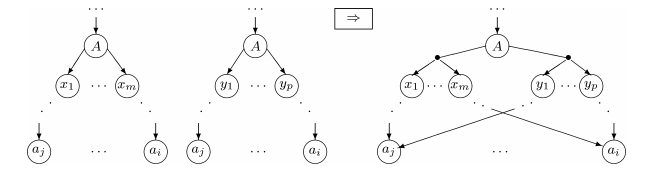
\includegraphics [width=0.8\linewidth] {sppf.PNG}}
\caption{Shared packed parse forest.}
\label{fig2}
\end{figure}

Для автоматического создания синтаксических анализаторов существует несколько подходов: можно полностью генерировать весь код парсера по грамматике, а потом использовать его. Чаще всего такой подход используется при генерации анализаторов, построенных методом рекурсивного спуска. При этом для каждого правила грамматики генерируются функции, которые последовательно вызываются в процессе работы парсера. Схема работы генератора при использовании данного подхода отображена на Рис.3.

\begin{figure}[h]
\center{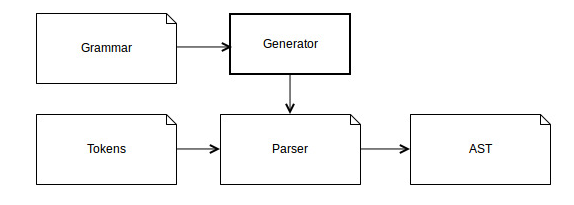
\includegraphics [width=0.9\linewidth] {figure1.PNG}}
\caption{Схема работы генератора синтаксических анализаторов при генерации всего кода парсера.}
\label{fig3}
\end{figure}

При другом подходе к автоматическому созданию парсеров генерируется только дополнительная необходимая для работы синтаксического анализатора информация, которая используется интерпретатором, содержащим в себе основную логику алгоритма. Чаще всего в качестве дополнительной информации генерируются управляющие таблицы, описанные выше, и информация о грамматике. Схема работы такого генератора отображена на Рис.4.

\begin{figure}[h]
\center{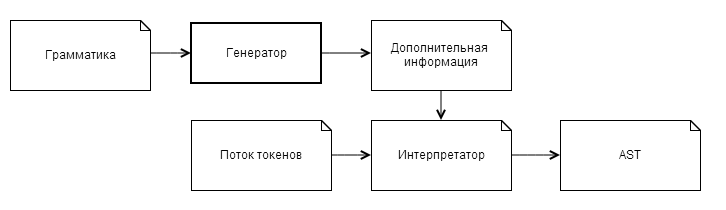
\includegraphics [width=1\linewidth] {ff.png}}
\caption{Схема работы генератора синтаксических анализаторов при генерации только дополнительной информации и использовании интерпретатора.}
\label{fig4}
\end{figure} 

Как упоминалось ранее, в реинжиниринге программного обеспечения важную роль играет синтаксический анализ. Современные инструменты позволяют генерировать синтаксические анализаторы по спецификации трансляции, но проекты, направленные на создание инструментов для автоматизации реинжиниринга программного обеспечения, выдвигают особые требования к генераторам синтаксических анализаторов[7]. Часто системы, подлежащие реинжинирингу, написаны на языках программирования, которые существовали ещё на заре развития теории синтаксически управляемой трансляции. По этой причине создание синтаксических анализаторов таких языков с помощью современных инструментов практически невозможно. Кроме того генераторы синтаксических анализаторов для реинжиниринга должны обрабатывать широкий класс языков, позволять разрешать неоднозначности в грамматике и порождать парсеры с высокой скоростью работы и хорошим механизмом восстановления после ошибок.

Этими свойствами обладает генератор синтаксических анализаторов для нужд автоматического реинжииринга программного обеспечения YaccConstructor[8], разрабатываемый на кафедре системного программирования Санкт-Петербургского государственного университета.

В процессе реинжиниринга грамматика часто подвергается изменениям, которые могут делать её неоднозначной и приводить к конфликтам, обработать которые возможно, используя восходящий алгоритм синтаксического анализа. Для обеспечения возможности работы с неоднозначными грамматиками в рамках проекта реализован GLR-генератор, порождающий восходящие парсеры с использованием алгоритма RNGLR[6], работающий со всеми контекстно-свободными грамматиками.

Кроме того в рамках проекта ведётся активная работа над абстрактным анализом встроенных языков. В отличие от классического анализа в абстрактном на вход анализатору подаётся не линейная последовательность символов, а некая структура, например граф. Данный подход позволяет производить статический анализ встроенных запросов. Например, если в коде встречается SQL-запрос, который собирается из строки, то обнаружить ошибку в таком запросе можно только в момент выполнения программы, что значительно замедляет процесс разработки и усложняет отладку. Также было бы удобно иметь возможность автодополнения и подсветки в таких запросах. Для работы с такими запросами и используется абстрактный анализ. 


Для создания абстрактных анализаторов чаще всего используется табличный подход. В статье [17] описан пример для создание табличного абстрактного анализатора на основе LR-таблиц. При этом не накладываются ограничения, из-за которых невозможно использовать LL-таблицы. В статье [18] описано решение, позволяющее создать абстрактный анализатор на основе обобщённого алгоритма RNGLR. В алгоритмах RNGLR [9] и GLL [18] процесс построения GSS и SPPF очень похож. По этой причине получение абстрактного анализатора на основе алгоритма GLL  представляется возможным. Его использование обладает следующими преимуществами:

\begin{itemize}
\item высокая скорость работы для леворекурсивных грамматик;
\item возможность более качественной и простой диагностики и восстановления от ошибок.
\end{itemize}

Именно это является главной причиной, по которой необходимо создать табличный анализатор с использованием алгоритма обобщённого нисходящего синтаксического анализа.

\section{Модуль генератора}
Ранее были описаны два основных подхода, используемые для автоматической генерации синтаксических анализаторов. Основными плюсами первого подхода, при котором генерируется весь кода парсера, является простота и удобство отладки таких парсеров. Несмотря на это в рамках проекта был создан генератор, использующий второй подход, - генерация дополнительной информации (функции для работы с грамматикой и управляющие таблицы). Выбор второго подхода обусловлен необходимостью получения абстрактного анализатора в дальнейшем, который в процессе работы использует таблицы предиктивного анализа.

На вход генератору подаётся грамматика, после чего она подвергается преобразованиям и представляется в компактном и удобном для работы виде.Для этой первичной обработки грамматики и её хранения переиспользуются модули из GLR-генератора.

После этого уже по преобразованной грамматике строится таблица, в ячейках которой хранятся номера продукций, по которым можно произвести разбор для текущего нетерминала и входного символа. В каждой ячейке такой таблицы может храниться несколько номеров продукций, что обусловлено возможным наличием неоднозначностей в грамматике. Данная таблица строится по аналогии с обычной LL-таблицей, с учётом того, что в грамматике могут быть неоднозначности.

Эта таблица, грамматика и функции для работы с ней в дальнейшем используются интерпретатором, который содержит в себе основную логику алгоритма GLL.
\section{Модуль интерпретатора}
\subsection{Модификации алгоритма GLL}

В статье, описывающей алгоритм [6], который взят за основу, по грамматике полностью генерируется синтаксический анализатор. Он состоит из набора функций для нетерминалов грамматики и управляющей функции. Управляющая функция контролирует процесс работы анализатора: извлекает новые дескрипторы (описатель текущего состояния) из очереди, присваивает необходимые значения и вызывает соответствующую функцию разбора.

Передача управления между функциями осуществляется с использованием команды goto. Поскольку в рамках работы необходимо реализовать табличный анализатор,  процесс работы которого отличается от описанного в статьях[10], в алгоритм были внесены некоторые изменения.

Вместо нескольких функций, соответствующих нетерминалам, используется пара функций: управляющая, которая выполняет ту же роль, что  и раньше,  и обрабатывающая. Для корректной работы обрабатывающей функции в зависимости от текущего входного символа и символа в грамматике были выделены следующие ситуации.

\begin{itemize}
\item Если текущий рассматриваемый символ х = А, где А --- терминал, то необходимо перейти к рассмотрению следующего символа в правиле, а указатель во входном потоке увеличить на единицу.
\item Если х --- это нетерминальный символ, то в стек записывается текущее правило и запоминается позиция в нём. С использованием этой информации будет осуществляться обработка после того, как нетерминал x будет обработан до конца. А рассматриваемым становится правило, по которому раскрывается х в зависимости от текущего символа во входном потоке. Указатель во входном потоке остается без изменений.
\item Если какое-то правило рассмотрено до конца и текущий стек не пуст, то извлекаем дескриптор с вершины стека и продолжаем работу с этими данными.
\end{itemize}

Таким образом обрабатывающая функция просто выполняет разные действия в зависимости от ситуации.

Для работы анализатора необходимы структуры, описывающие деревья вывода и стек. Как упоминалось ранее, процесс работы с такими структурами в алгоритмах GLL и RNGLR похож. Поэтому в ходе разработки GLL-модуля эти структуры переиспользовались без изменений. 

\subsection{Тестирование}

Результатом работы интерпретатора является абстрактное синтаксическое дерево, для представления которого используется SPPF. Например, рассмотрим простую грамматику, содержашую неоднозначность:
\begin{center}
    s := A d B | A D B
    \\d := D
\end{center}

Для такой грамматики и входа ADB дерево отображено на Рис. ~\ref{fig8}.

В этом дереве помечен нетерминал, разбор которого может быть произведён двумя разными способами: с помощью продукции s := A d B и s := A D B. При этом терминальные ячейки, которые являются листьями, хранятся в единственном экземпляре в данном случае, т.е. каждая такая ячейка для данной позиции во входном потоке создаётся лишь однажды, а потом переиспользуется.

Рассмотрим леворекурсивную грамматику $H_4$:
\begin{center}
    s := B | s s
\end{center}

Для такой грамматики и входа BBB дерево будет иметь вид как на  Рис. ~\ref{fig9}.


\begin{figure}[h]
\center{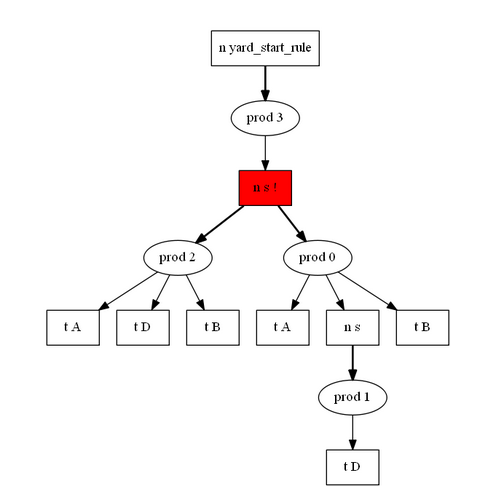
\includegraphics [width=0.4\linewidth] {tree2.PNG}}
\caption{Дерево вывода для грамматики $H_3$ и входа ADВ.}
\label{fig8}
\end{figure}
\pagebreak
\begin{figure}[h]
\center{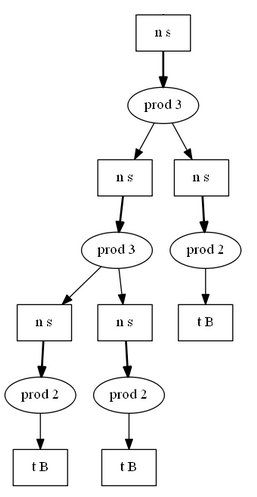
\includegraphics [width=0.4\linewidth] {tree3.PNG}}
\caption{Дерево вывода для грамматики $H_4$ и входа BBB.}
\label{fig9}
\end{figure}

\section{Анализ и сравнение}
Основным достоинством GLL является обработка левой и скрытой левой рекурсии. Для демонстрации преимуществ GLL были выбраны соответствующие грамматики и проведено сравнение времени работы с уже существующей реализацией RNGLR. 

Для экспериментов использовалась леворекурсивная грамматика $H_4$ следующего вида:
\begin{center}
    s := B | s s
\end{center}

На вход подавались последовательности из токенов B с шагом 10. В ходе экспериментов были получены следующие результаты:

\begin{figure}[h]
\center{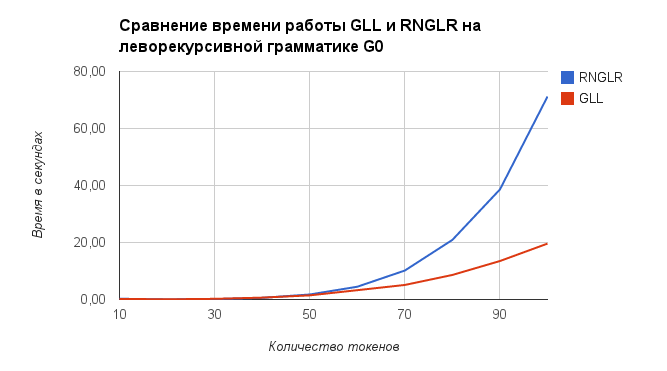
\includegraphics [width=0.7\linewidth] {chart1.png}}
\caption{Результаты сравнения для леворекурсивной грамматики $H_4$.}
\label{fig11}
\end{figure}

Также были проведены эксперименты для грамматики $H_5$ со скрытой левой рекурсией:
\begin{center}
    s := B | (f A)
    \\f := s s
\end{center}
	
Для замеров использовались входные цепочки из токенов B с шагом 10 и токеном A на конце, то есть цепочки вида $B^(n*10)$A. Были получены следующие результаты:

\begin{figure}[h]
\center{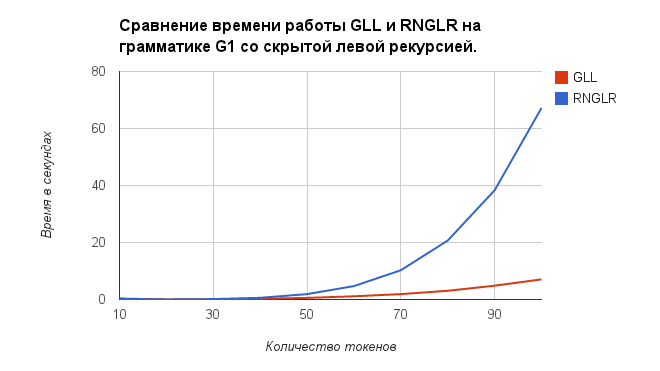
\includegraphics [width=0.7\linewidth] {chart2.png}}
\caption{Результаты сравнения для леворекурсивной грамматики $H_5$.}
\label{fig12}
\end{figure}

Из экспериментов видно, что GLL грамматики с левой и скрытой левой рекурсией быстрее RNGLR.

\section*{Заключение}
В ходе данной работы получены следующие результаты.
\begin{itemize}
\item В проекте YC реализован генератор табличных GLL анализаторов.
\item В проекте YC реализован алгоритм табличного GLL анализа. В отличии от ранее описанного GLL анализа, использующего явную генерацию в код, табличный подход предоставляет возможность использовать данный алгоритм для абстрактного анализа.
\item Продемонстрирована работоспособность реализованного алгоритма для основных сценариев: неоднозначная грамматика, грамматика с левой рекурсией и грамматика со скрытой левой рекурсией.
\item Проведено сравнение производительности реализованного GLL-анализатора с уже существовавшим и использующимся в промышленных проектах RNGLR-анализатором.
\end{itemize}

В процессе разработки происходила активная интеграция с уже существующим GLR-модулем, о котором упоминалось выше, и многие структуры переиспользовались.

Также было принято участие во Всероссийской научной конференции по проблемам информатики “СПИСОК” и Software Engineering Colloquium SYRCoSE. 

В ходе работы был получен табличный GLL-анализатор. Преобразование из явной генерации кода в табличный анализ потребовало обобщения  и существенной модификации алгоритма, описанного в существующих работах. В дальнейшем необходимо провести более полное тестирование и создать подробное описание реализованных обобщённых функций. 
Отдельной большой задачей является реализация абстрактного GLL-анализа --- механизма анализа для встроенных языков, для чего и потребовалась табличная версия алгоритма. Для этого, что будет полезно и само по себе, необходимо расширить алгоритм механизмом восстановления после ошибок и реализовать непосредственную поддержку EBNF.
 

\begin{thebibliography}{99}

\bibitem{ulman}  
Alfred V.~Aho and Ullman, \emph{The Theory of Parsing, Translation and Compiling}, Parsing of Series in Automatic Computation. \relax Prentice-Hall, 1972. P. 33-45.

\bibitem{aho}
Alfred V. Aho, Monica S. Lam, Ravi Sethi, and Jeffrey D. Ullman, Compilers: Principles, Techniques and Tools. Pearson Education, Inc, 2006.

\bibitem{Rosenkrantz}
D.J. Rosenkrantz and R.E. Stearns. Proceeding STOC '69 Proceedings of the first annual ACM symposium on Theory of computing. ACM, 1969. P. 165-180.

\bibitem{grune}
Dick Grune and J. H. Ceriel Jacobs. Parsing Techniques: A Practical Guide (Second Edition). Springer, 2008.

\bibitem{grune2}
Dick Grune, Kees van Reeuwijk, Henri E. Bal, Ceriel J.H. Jacobs, and Koen G. Langendoen. Modern Compiler Design (Second Edition). John Wiley \& Sons, 2010.

\bibitem{gll}
Elizabeth Scott and Adrian Johnstone GLL Parsing. Electronic Notes in Theoretical Computer Science 253, 2010. P. 177-189.

\bibitem{kirilenko}
Y.A. Kirilenko, S.V. Grigoriev, D.A. Avdyukhin. Syntax analyzers development in automated reengineering of informational system. Scientific and technical statements SPbSPU Issue 3, 2013.

\bibitem{yc}
\relax YaccConstructor home page https://code.google.com/p/recursive-ascent/wiki/YaccConstructor

\bibitem{rnglr}
Elizabeth Scott and Adrian Johnstone. Right Nulled GLR Parsers.

\bibitem{implementation}
Elizabeth Scott and Adrian Johnstone. Modelling GLL Parser Implementations. Engineering Lecture Notes in Computer Science Volume 6563, 2011. P. 42-61.

\bibitem{tomita}
Masaru Tomita. Generalized LR parsing. Kluwer academic publishers, 1991.

\bibitem{earley}
J. Aycock and N. Horspool. Practical Earley Parsing. The Computer Journal, P. 620–630, 2002.

\bibitem{earley2}
J. Earley. An Efficient Context-Free Parsing Algorithm. Commun. ACM, P. 94–102, 1970.

\bibitem{rekers}
REKERS, J. G. 1992. Parser generation for interactive environments. Ph.D. thesis, Universty of Amsterdam.

\bibitem{tomita2}
Masaru Tomita. Eficient parsing for natural language: a fast algorithm for practical systems. Kluwer Academic Publishers, Boston, 1986.

\bibitem{antlr}
Официальный сайт ANTLR http://www.antlr.org/.

\bibitem{abstrParse}
Kyung-Goo Doh, Hyunha Kim, and David A. Schmidt: Abstract parsing: Static analysis of dynamically generated string output using lr-parsing technology. In Proceedings of the 16th International Symposium on Static Analysis, SAS ’09. Springer-Verlag: Berlin; Heidelberg, 2009. P. 256–272.

\bibitem{abstrParse2}
Grigoriev Semyon, Kirilenko Iakov. GLR-based abstract parsing // CEE-SECR’13 Proceedings of the 9th Central & Eastern European Software Engineering Conference in Russia.

\bibitem{treeGeneration}
Elizabeth Scott, Adrian Johnstone. GLL parse-tree generation. Science of Computer Programming, Volume 78, Issue 10, 2013, P. 1828–1844.
\end{thebibliography}
